\documentclass[11pt,a4paper]{article}
\usepackage[utf8]{inputenc}
\usepackage{amsmath}
\usepackage{mathtools}
\usepackage{amsfonts}
\usepackage{amssymb}
\usepackage{graphicx}
\usepackage{caption}
\usepackage{subcaption}
\usepackage{comment}
\usepackage{color}
\usepackage{enumitem}
\usepackage[left=2cm,right=2cm,top=2cm,bottom=2cm]{geometry}
\usepackage{listings}
\usepackage{color}

\setlength{\jot}{10pt}
 
\definecolor{codegreen}{rgb}{0,0.6,0}
\definecolor{codegray}{rgb}{0.5,0.5,0.5}
\definecolor{codepurple}{rgb}{0.58,0,0.82}
\definecolor{backcolour}{rgb}{0.95,0.95,0.92}
 
\lstdefinestyle{mystyle}{
    backgroundcolor=\color{backcolour},   
    commentstyle=\color{codegreen},
    keywordstyle=\color{magenta},
    numberstyle=\tiny\color{codegray},
    stringstyle=\color{codepurple},
    basicstyle=\footnotesize,
    breakatwhitespace=false,         
    breaklines=true,                 
    captionpos=b,                    
    keepspaces=true,                 
    numbers=left,                    
    numbersep=5pt,                  
    showspaces=false,                
    showstringspaces=false,
    showtabs=false,                  
    tabsize=2
}
 
\lstset{style=mystyle}
\author{Andrew Teta}
\title{ECEN 4532 - Lab 2: Introduction to Image Processing}

\begin{document}

\maketitle

\begin{figure}[ht]
	\centering
	\begin{subfigure}[h]{0.6\textwidth}
		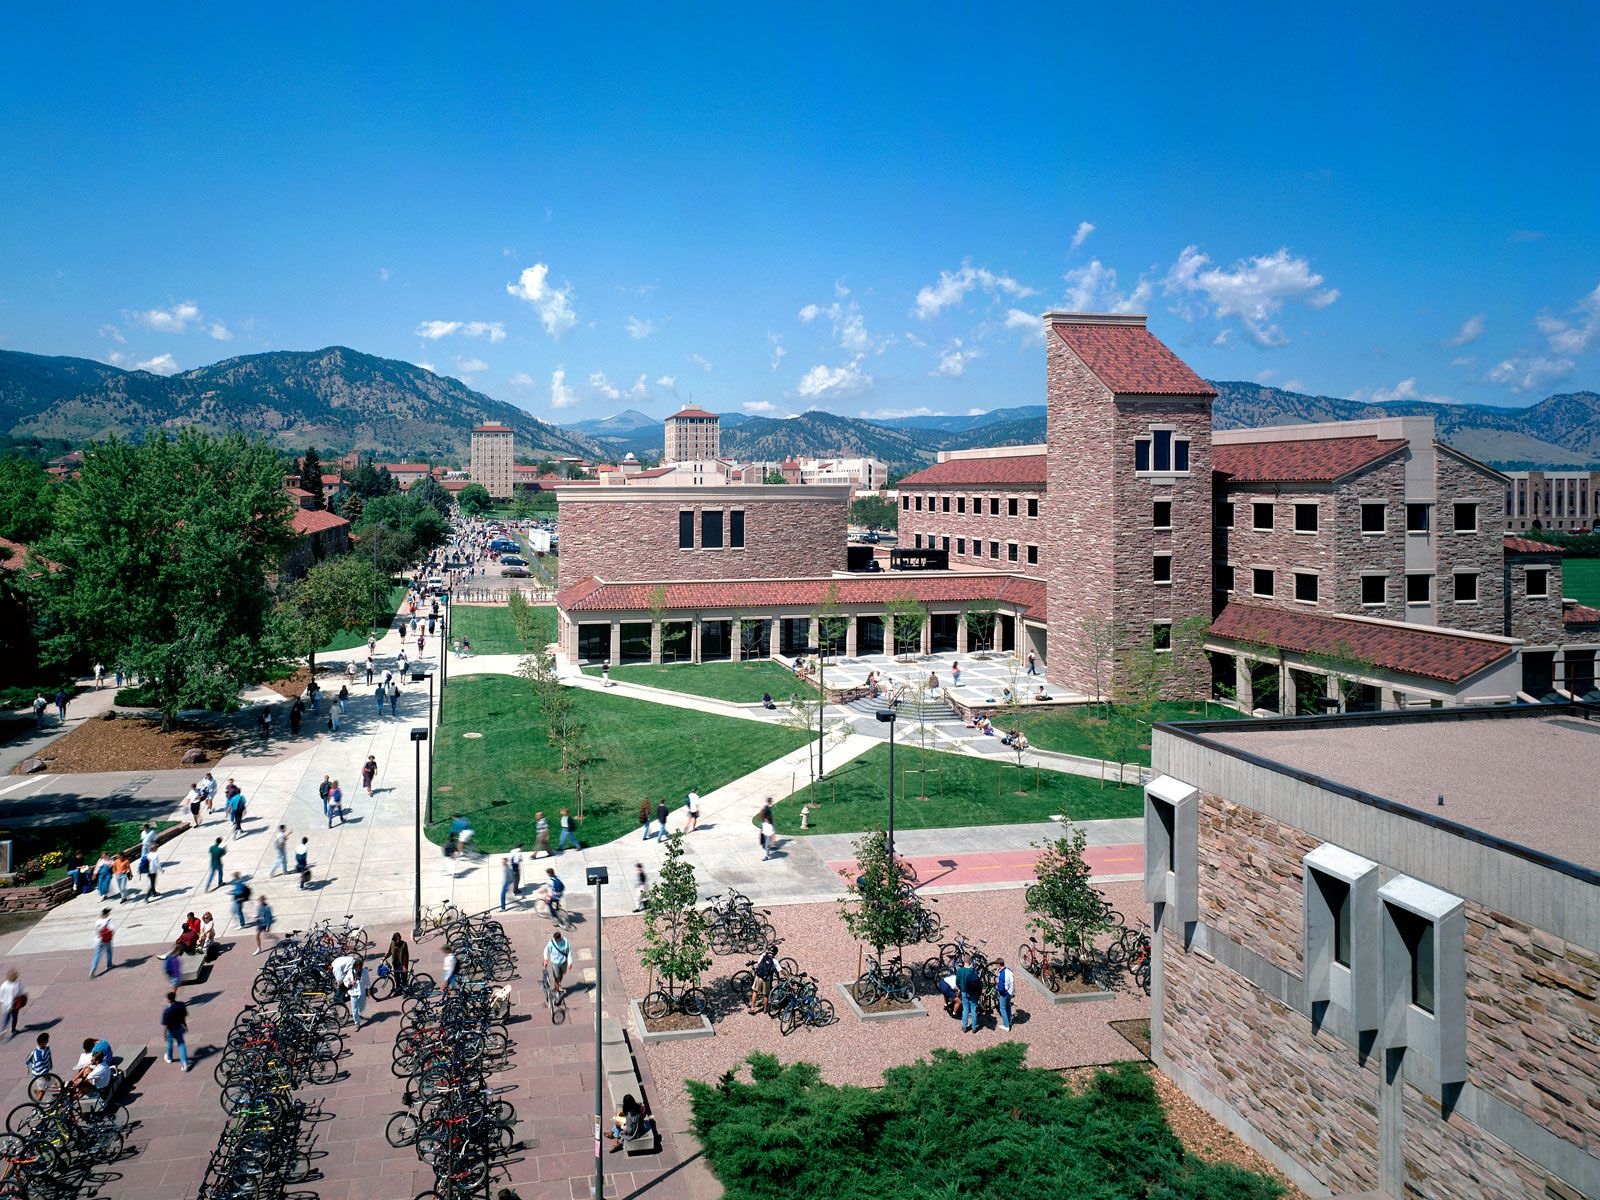
\includegraphics[width=\textwidth]{images/test01}
	\end{subfigure}
	\begin{subfigure}[h]{0.6\textwidth}
		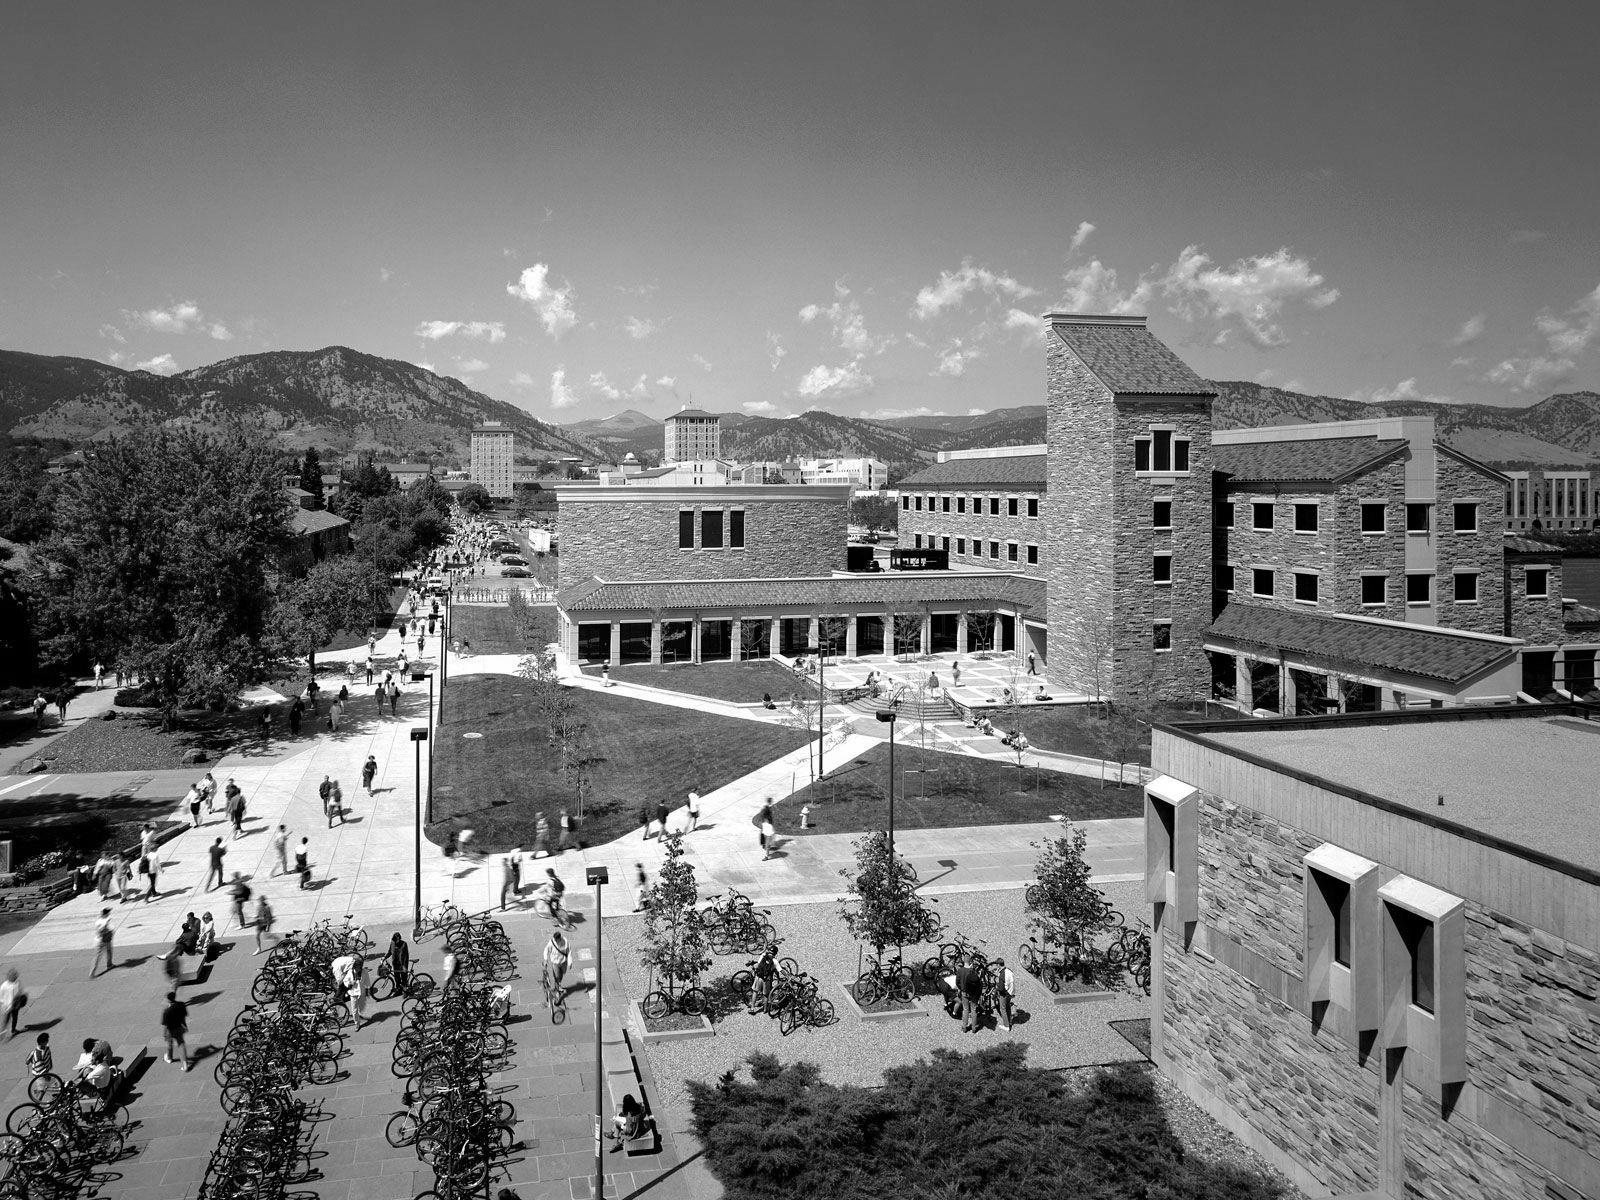
\includegraphics[width=\textwidth]{figs/test01_gray}
	\end{subfigure}
\end{figure}

\pagebreak

\tableofcontents

\pagebreak

\addcontentsline{toc}{section}{Introduction}
\section{Introduction}
\paragraph*{} In this discussion, we will be exploring some common manipulations applied to images as an introduction to image processing. The analysis will be performed in Python, using a few libraries such as \verb|Pillow| for basic image file manipulations (opening, saving), \verb|numpy| for efficient array operations, \verb|scipy.signal| for some Fourier functionality, \verb|scipy.interpolate| for interpolation, \\ \verb|collections.Counter| to count occurrences of multiple values in a list, and \verb|matplotlib.pyplot| for basic plotting. We will use functions from these libraries to help perform grayscale conversion, contrast enhancement, edge detection, and image resizing, although most of the code for these will be developed from scratch.

\addcontentsline{toc}{subsection}{Background}

\subsection{Background}
\paragraph*{} We will be working with a common uncompressed image format, BMP (short for bitmap). This file type begins with a short header, followed by a 2-dimensional array of pixel information. Color BMP files store three 8-bit numbers for each pixel, corresponding to an R, G, and B intensity value.

\begin{figure}
	\centering
	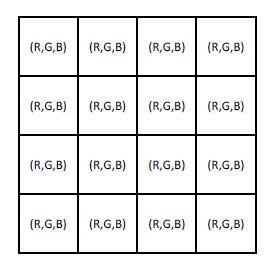
\includegraphics[width=0.5\textwidth]{figs/rgb_example}
	\caption{Example of a 4x4 color BMP image file}
	\label{fig:rgb_example}
\end{figure}

Different combinations of the three chroma values produce unique colors. Given 8-bit color depth, it is possible to represent $2^{24}$ colors.
\paragraph*{} In this lab, we will only be processing monochromatic (grayscale) images, with only 8 bits per pixel (0=black, 255=white). This will simplify analysis. The monochrome value associated with a pixel can be found from its RGB values using a dot product

\begin{equation} \label{eq:Y}
Y = (0.299,0.587,0.114)\cdot(R,G,B)
\end{equation}

\paragraph*{} The BMP header encodes image size and some other metadata. We will use \verb|Pillow| to import and export images in Python. \verb|Pillow| basically converts the input image to a BMP format when \verb|open()| is called.

\pagebreak

\section{Grayscale Conversion}
\subsection{Introduction} In many image processing tasks, color is unnecessary. Converting between color spaces (there are more than just grayscale and RGB) can be done using a matrix multiplication. YUV is a common matrix to use, found in TV applications (Y represents luminosity).

\begin{equation}\label{eq:YUV}
     \begin{bmatrix}
       Y \\
       U \\
       V
     \end{bmatrix}
     =
     \begin{bmatrix}
       0.299 & 0.587 & 0.114 \\
       -0.14713 & -0.28886 & 0.436 \\
       0.615 & -0.51499 & -0.10001
     \end{bmatrix}
     \begin{bmatrix}
       R \\
       G \\
       B
     \end{bmatrix}
\end{equation}

U and V are color difference signals and can be positive or negative, while Y ranges from 0 to 255.

\subsection{Method} We will use \verb|Pillow| for image input/output in Python. Importing an image will also involve converting it into a \verb|numpy| array for processing. The basic implementation is to open the file, convert it to a \verb|numpy| array, take the dot product of the Y vector and the image (as in eq. \ref{eq:Y}), and clip out-of-range values. See \ref{app:gray} for the full implementation.

\subsection{Results} Two images before and after grayscale conversion are shown below. 

\begin{figure}[ht]
	\centering
	\begin{subfigure}[h]{0.45\textwidth}
		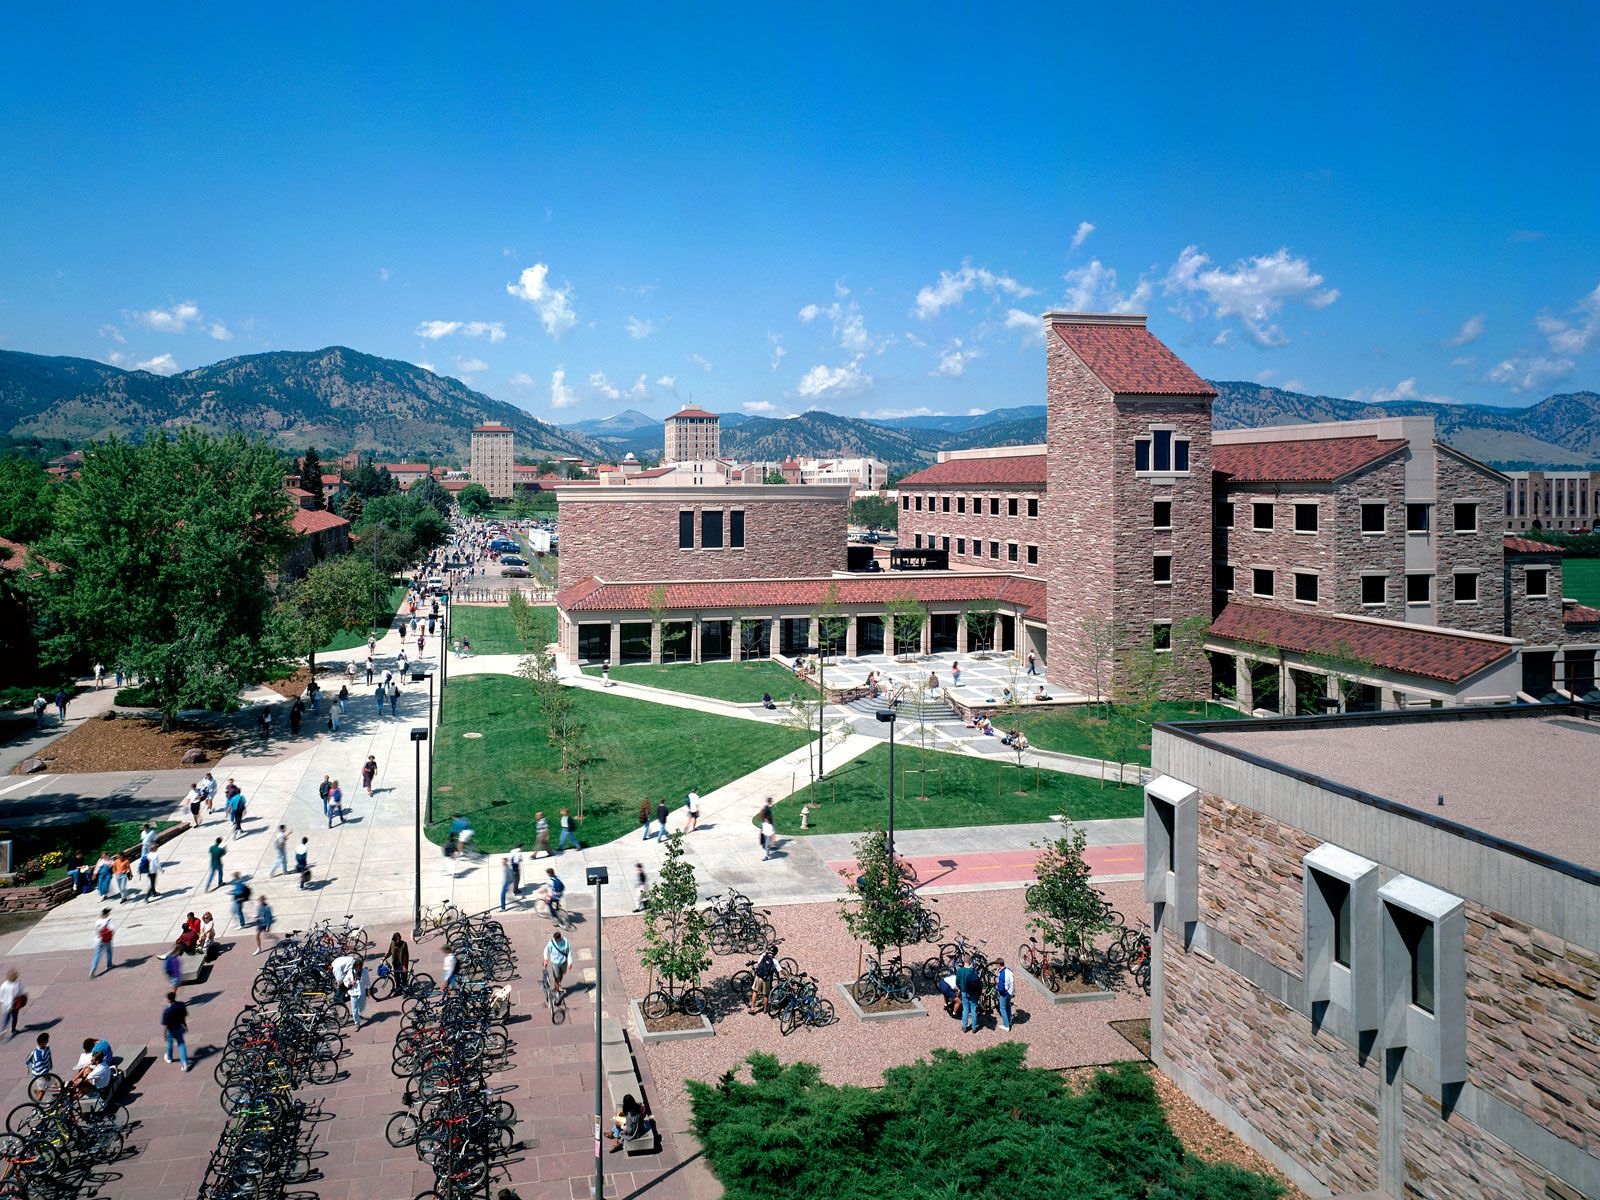
\includegraphics[width=\textwidth]{images/test01}
		\caption{Before}
		\label{fig:gray1_bef}
	\end{subfigure}
	\begin{subfigure}[h]{0.45\textwidth}
		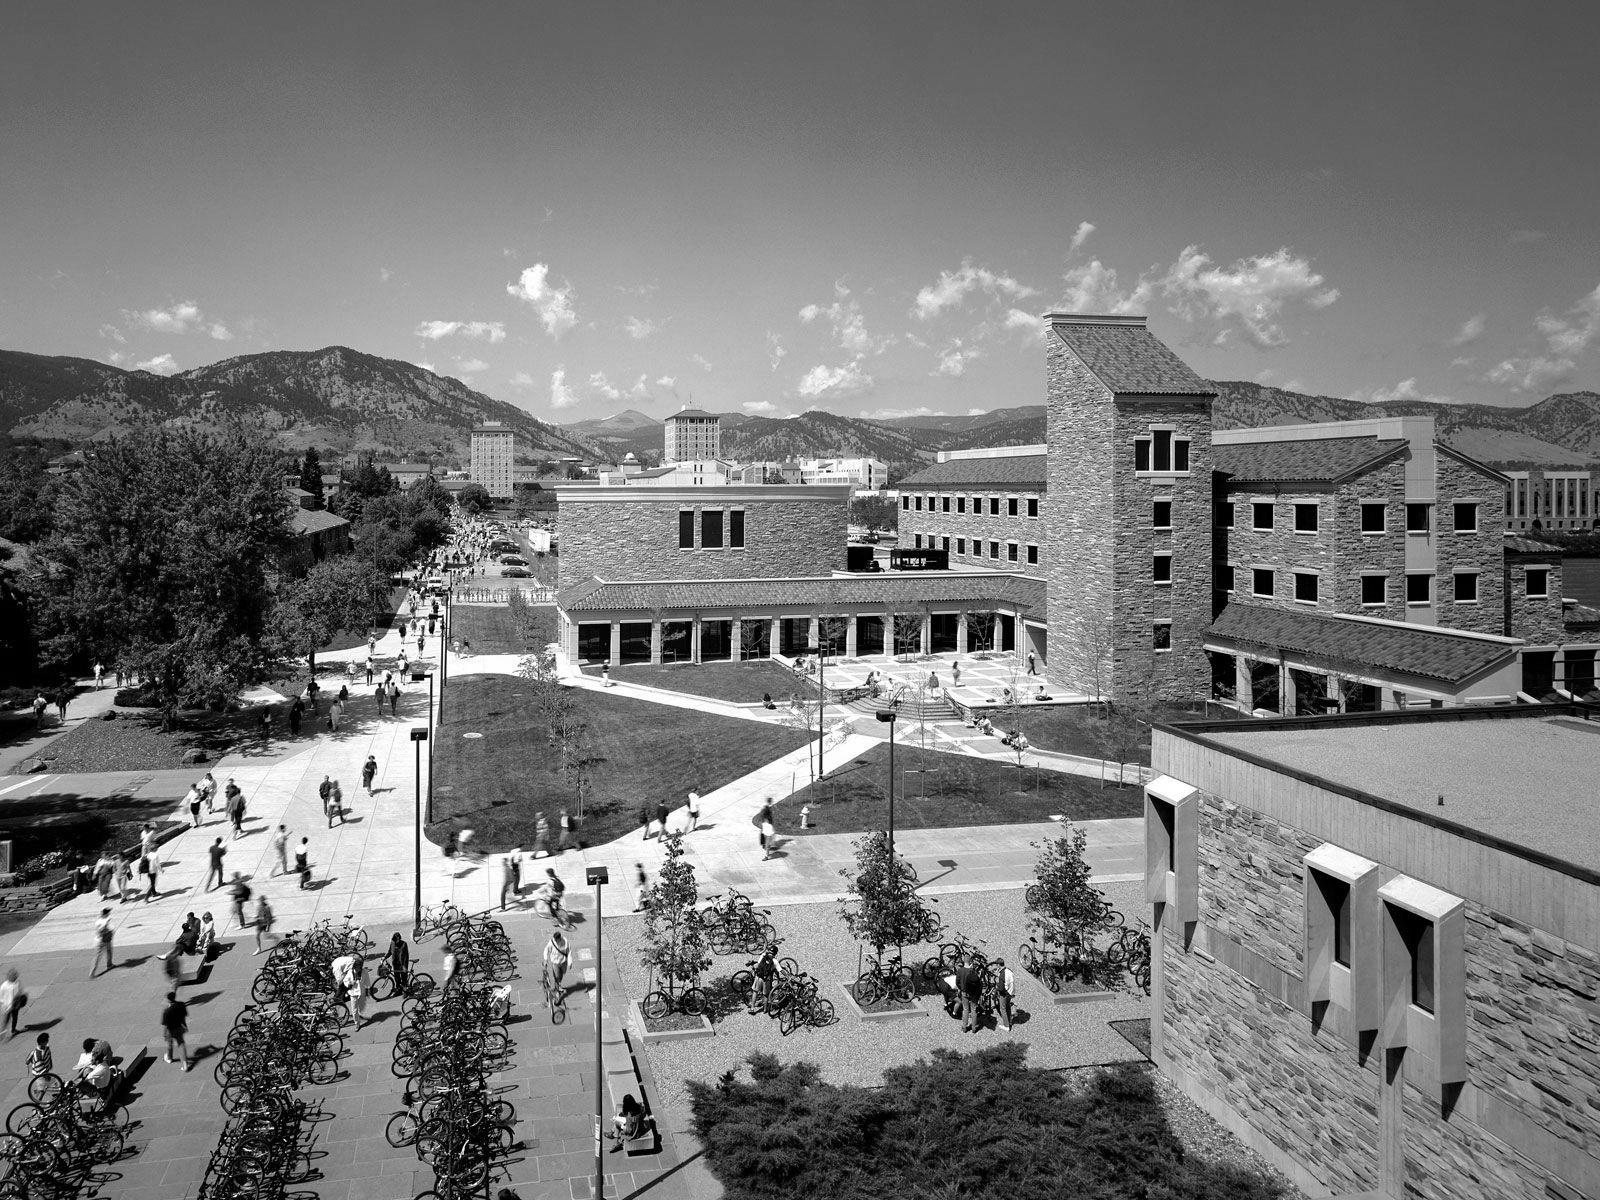
\includegraphics[width=\textwidth]{figs/test01_gray}
		\caption{After}
		\label{fig:gray1_aft}
	\end{subfigure}
	\caption{A picture of the Math building on CU Boulder campus before and after grayscale conversion.}
	\label{fig:gray1}
\end{figure}

\begin{figure}[ht]
	\centering
	\begin{subfigure}[h]{0.45\textwidth}
		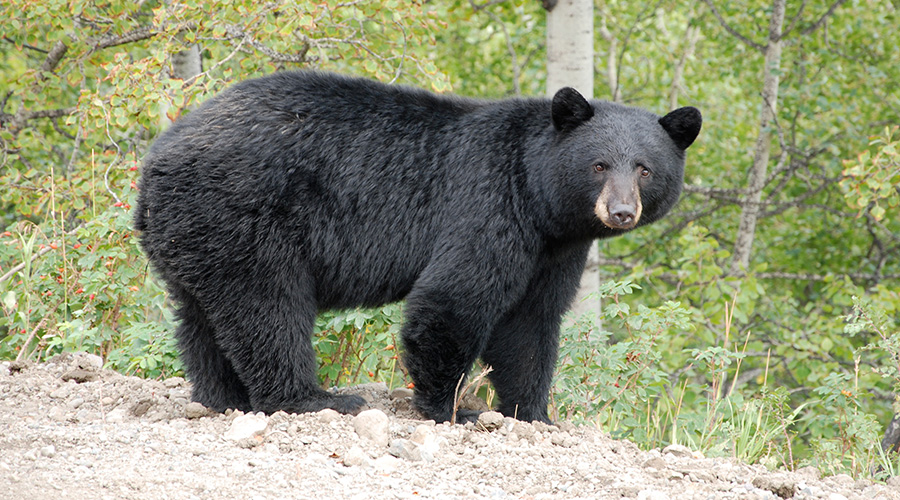
\includegraphics[width=\textwidth]{images/test02}
		\caption{Before}
		\label{fig:gray2_bef}
	\end{subfigure}
	\begin{subfigure}[h]{0.45\textwidth}
		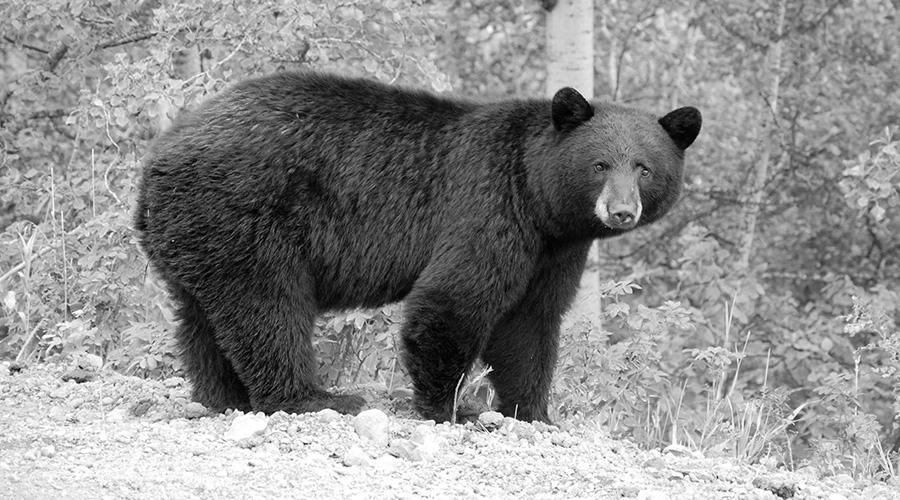
\includegraphics[width=\textwidth]{figs/test02_gray}
		\caption{After}
		\label{fig:gray2_aft}
	\end{subfigure}
	\caption{A picture of a bear before and after grayscale conversion.}
	\label{fig:gray2}
\end{figure}

\clearpage

\section{Contrast Enhancement}

\subsection{Introduction}
Sometimes a picture will have low dynamic range and appears low contrast. A simple contrast enhancement process based on \textit{histogram equalization} can make a huge improvement. In this part of the lab, we will be implementing histogram equalization as a contrast enhancement algorithm. This means that we will take an image with tightly grouped intensities and try to 'equalize' it so that the intensities are evenly distributed.

\subsection{Method} 
We begin by opening an image and converting it to grayscale, using the \verb|Pillow| function, \verb|convert('L')|. Then, we can use \verb|collections.Counter| to find the number of occurrences of each intensity value. \verb|Counter| returns an array of the values, but is structured like a dictionary and is not sorted. Thus, looping over intensity (0 to 255) we can extract the frequencies in a sorted \verb|numpy| array.

\begin{lstlisting}[language=Python]
image = image.convert('L')
image = np.asarray(image, np.float)
hist_before = np.zeros(256, dtype=int)
freq = Counter(np.reshape(image, image.shape[0] * image.shape[1]))
for p in range(256):
    hist_before[p] = freq[p]
\end{lstlisting}

At this point, \verb|hist_before| holds a histogram of intensity.

\begin{figure}[ht]
	\centering
	\begin{subfigure}[h]{0.45\textwidth}
		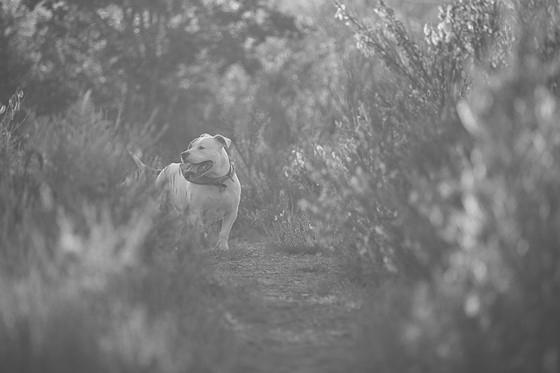
\includegraphics[width=\textwidth]{figs/lc1_gray}
		\caption{A low-contrast image.}
		\label{fig:gray_lc1}
	\end{subfigure}
	\begin{subfigure}[h]{0.45\textwidth}
		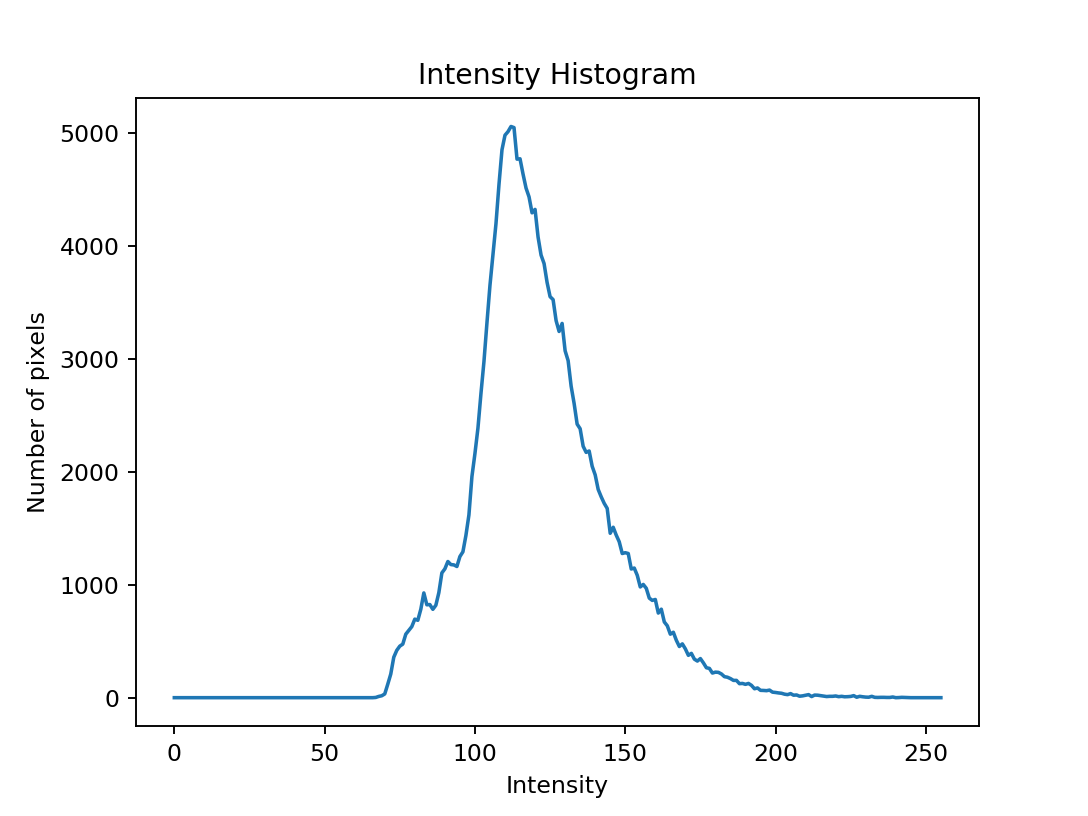
\includegraphics[width=\textwidth]{figs/lc1_hist_bef}
		\caption{Intensity histogram.}
		\label{fig:lc1_hist_bef}
	\end{subfigure}
	\caption{Intensity histogram of a low contrast image. Note the lack of any values on the low or high end of the spectrum. This is what makes it low contrast, as there is low dynamic range.}
	\label{fig:lc1_hist}
\end{figure}

Next, we want to find a function to map intensities of one value to another in a way that will 'equalize' the histogram in figure \ref{fig:lc1_hist_bef}.
We wish to remap the intensities of the original image, so that each intensity occurs with the same frequency. Then the ideal pixel count for any given intensity would be $P = (total \# of pixels) / (number of intensity values)$. We will ignore values of 0 or 255 as they cannot be remapped to anything except themselves. Looping over intensity (1 to 254), we hold a running sum, counting the number of pixels that have been remapped in a variable \verb|curr_sum|. Initially, we find pixels to be remapped to a value of 1. We do this until we've remapped at least as many pixels as we had aimed for. Then, we start mapping to a new value, determined by \verb|round(curr_sum/P)|, which accounts for some overshoot.

\begin{lstlisting}[language=Python]
remap = np.zeros(256, dtype=int)
remap[-1] = 255
histSum = sum(hist_before[1:-2])
P = histSum / 254
T = P
outval = 1
curr_sum = 0
# build remap table
for inval in range(1, 255, 1):
    curr_sum += hist_before[inval]
    remap[inval] = outval
    if (curr_sum > T):
        outval = round(curr_sum/P)
        T = outval*P
\end{lstlisting}

\begin{figure}[ht]
	\centering
	\begin{subfigure}[h]{0.45\textwidth}
		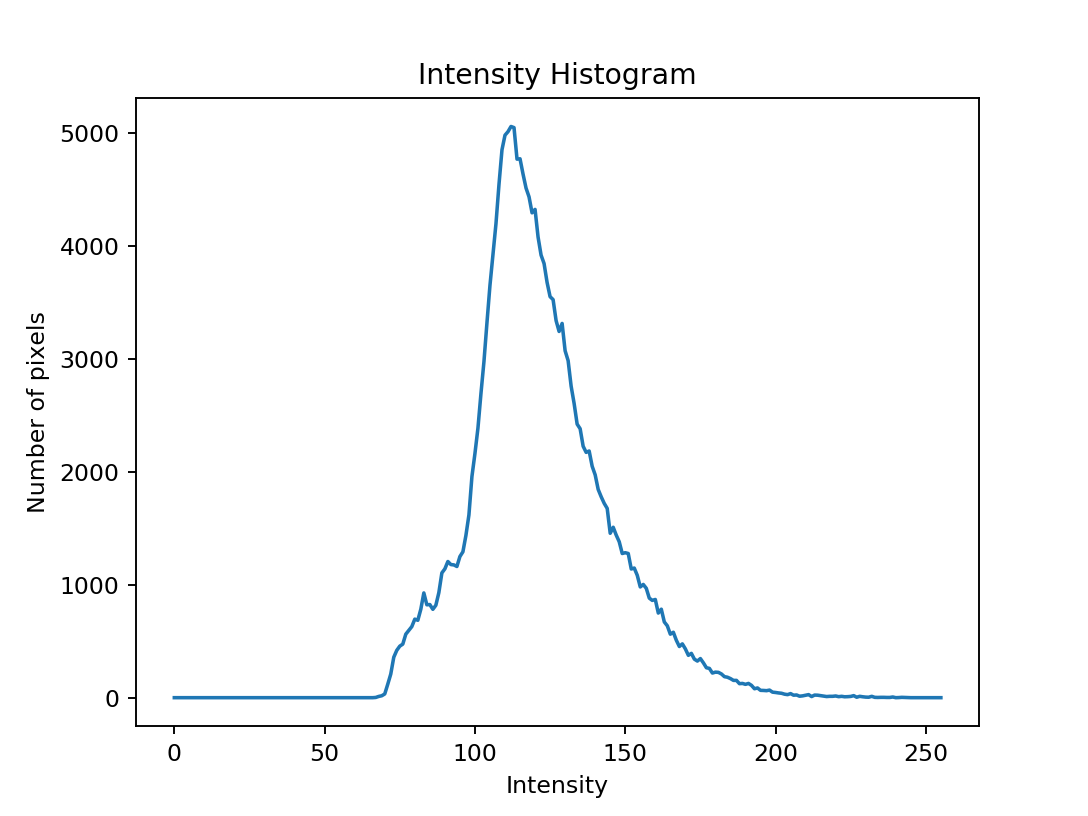
\includegraphics[width=\textwidth]{figs/lc1_hist_bef}
		\caption{histogram of low-contrast image}
		\label{fig:lc1_hist_before_r}
	\end{subfigure}
	\begin{subfigure}[h]{0.45\textwidth}
		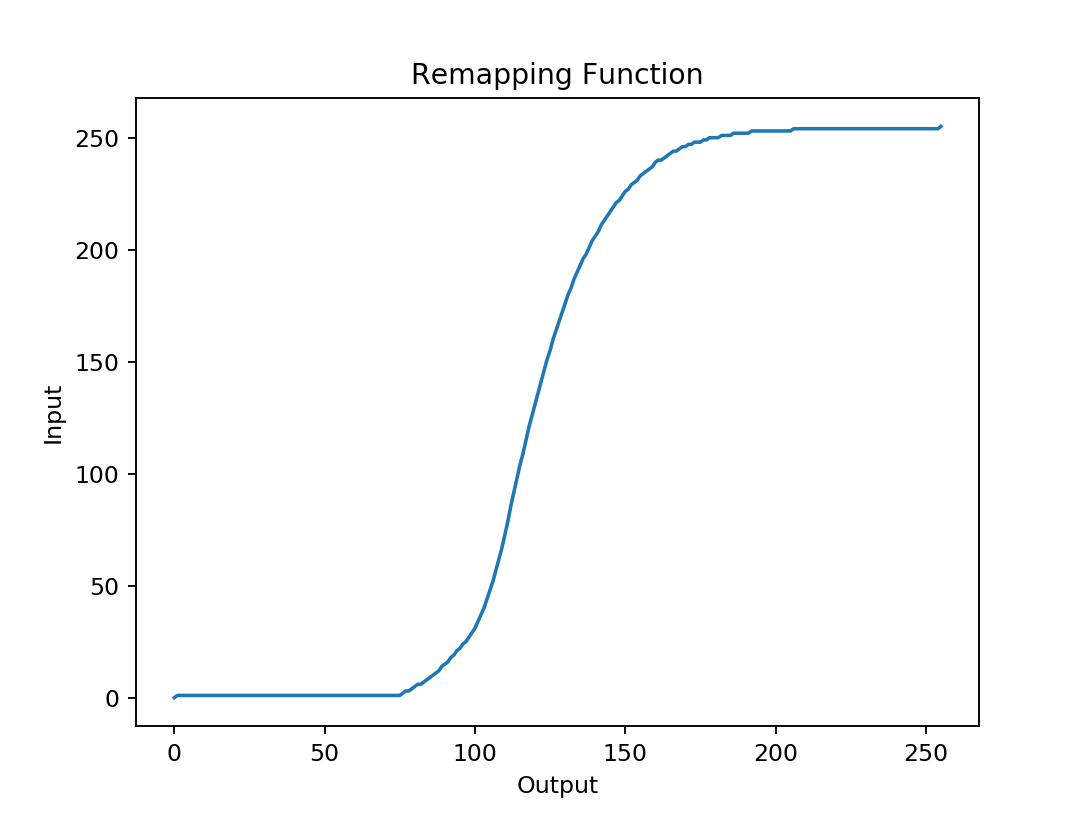
\includegraphics[width=\textwidth]{figs/lc1_remap}
		\caption{remapping function}
		\label{fig:lc1_remap}
	\end{subfigure}
	\caption{Histogram and remapping function for a low contrast image.}
	\label{fig:lc1_remap_func}
\end{figure}

Figure \ref{fig:lc1_remap} shows how intensity values are remapped for the image in \ref{fig:gray_lc1}. Notice that many of the pixel intensities centered around the middle will be spread out to occupy most of the spectrum.
Next, we need to apply the remapping function to the image and produce the contrast-enhanced picture. To do this, we will use \verb|numpy.where|.

\begin{lstlisting}[language=Python]
image_equalized = np.zeros_like(image)
for intensity in range(256):
    image_equalized = np.where(image == intensity, remap[intensity], image_equalized)
\end{lstlisting}

\subsection{Results}
The full results of contrast enhancement for two images can be seen in figures \ref{fig:eq1} and \ref{fig:eq2}.

\begin{figure}[h]
	\ContinuedFloat*
	\centering
	\begin{subfigure}[h]{0.7\textwidth}
		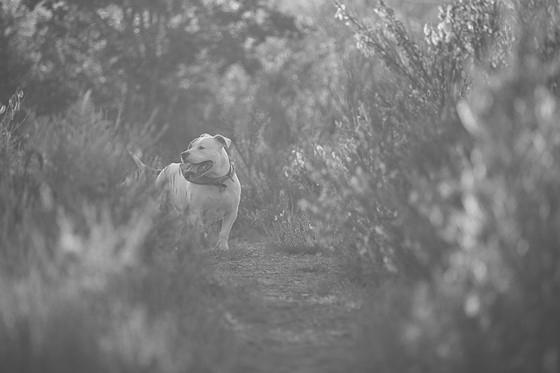
\includegraphics[width=\textwidth]{figs/lc1_gray}
		\caption{original}
		\label{fig:lc1_orig}
	\end{subfigure}
	
	\begin{subfigure}[h]{0.75\textwidth}
		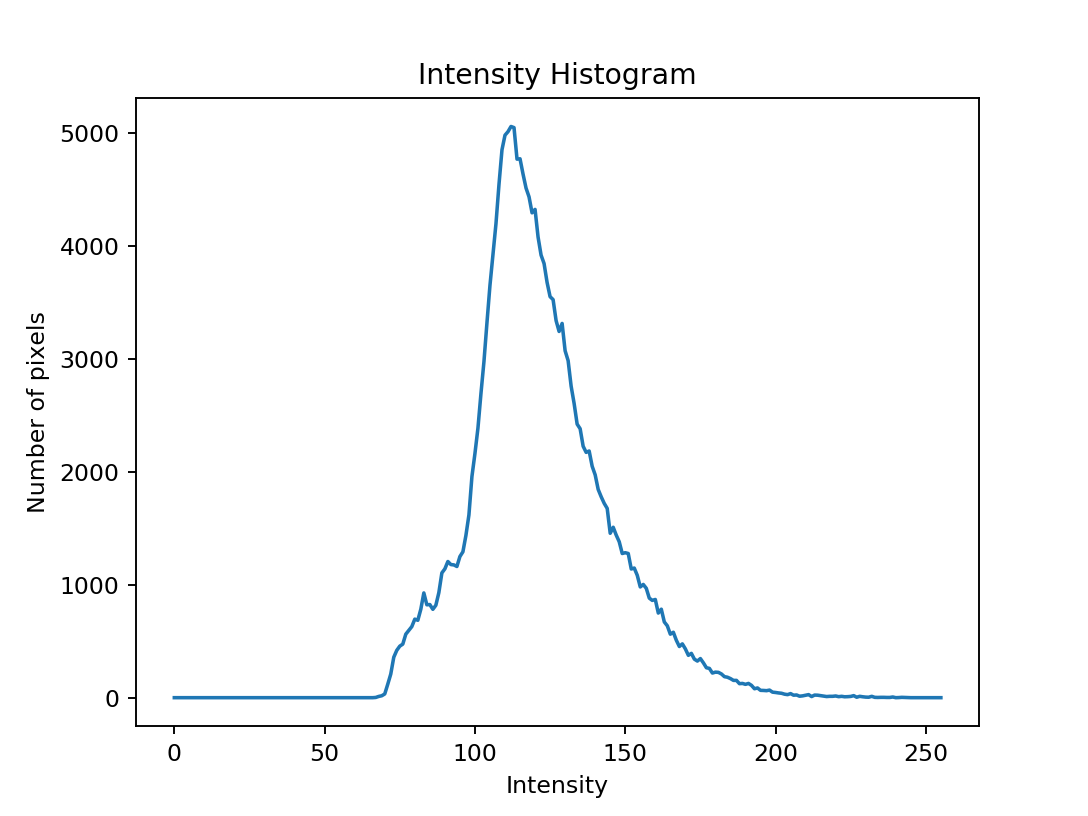
\includegraphics[width=\textwidth]{figs/lc1_hist_bef}
		\caption{before}
		\label{fig:hist_bef_1}
	\end{subfigure}
	
	\caption{Contrast enhancement.}
	\label{fig:eq1}
\end{figure}

\clearpage

\begin{figure}[h]
	\ContinuedFloat
	\centering
	\begin{subfigure}[h]{0.7\textwidth}
		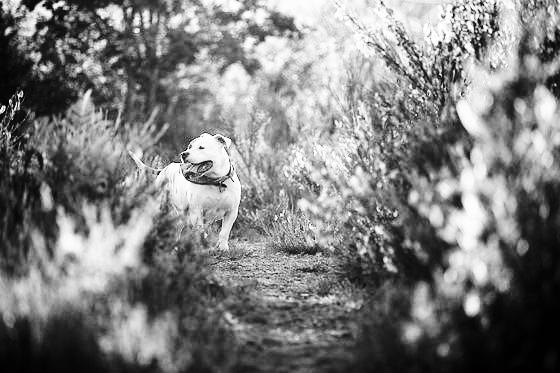
\includegraphics[width=\textwidth]{figs/lc1_ce}
		\caption{contrast enhanced}
		\label{fig:lc1_after}
	\end{subfigure}
	
	\begin{subfigure}[h]{0.75\textwidth}
		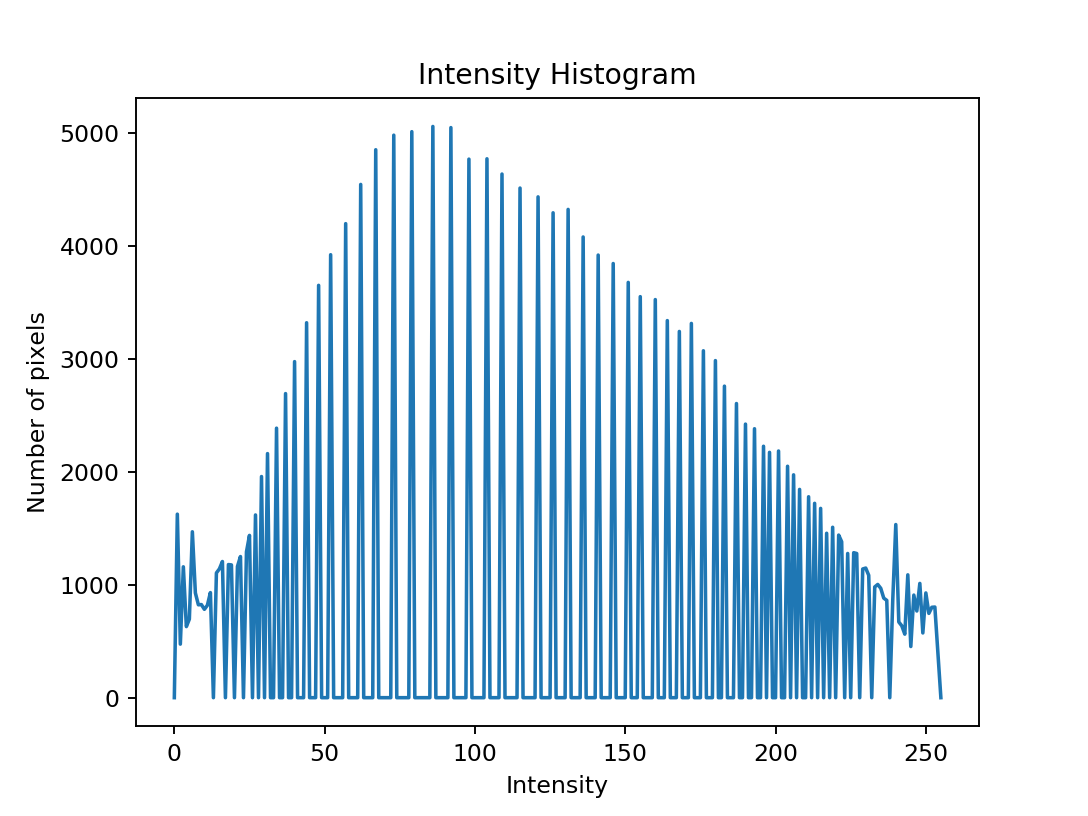
\includegraphics[width=\textwidth]{figs/lc1_hist_aft}
		\caption{after}
		\label{fig:hist_aft_1}
	\end{subfigure}
\end{figure}

\clearpage

\begin{figure}[h]
	\ContinuedFloat*
	\centering
	\begin{subfigure}[h]{0.7\textwidth}
		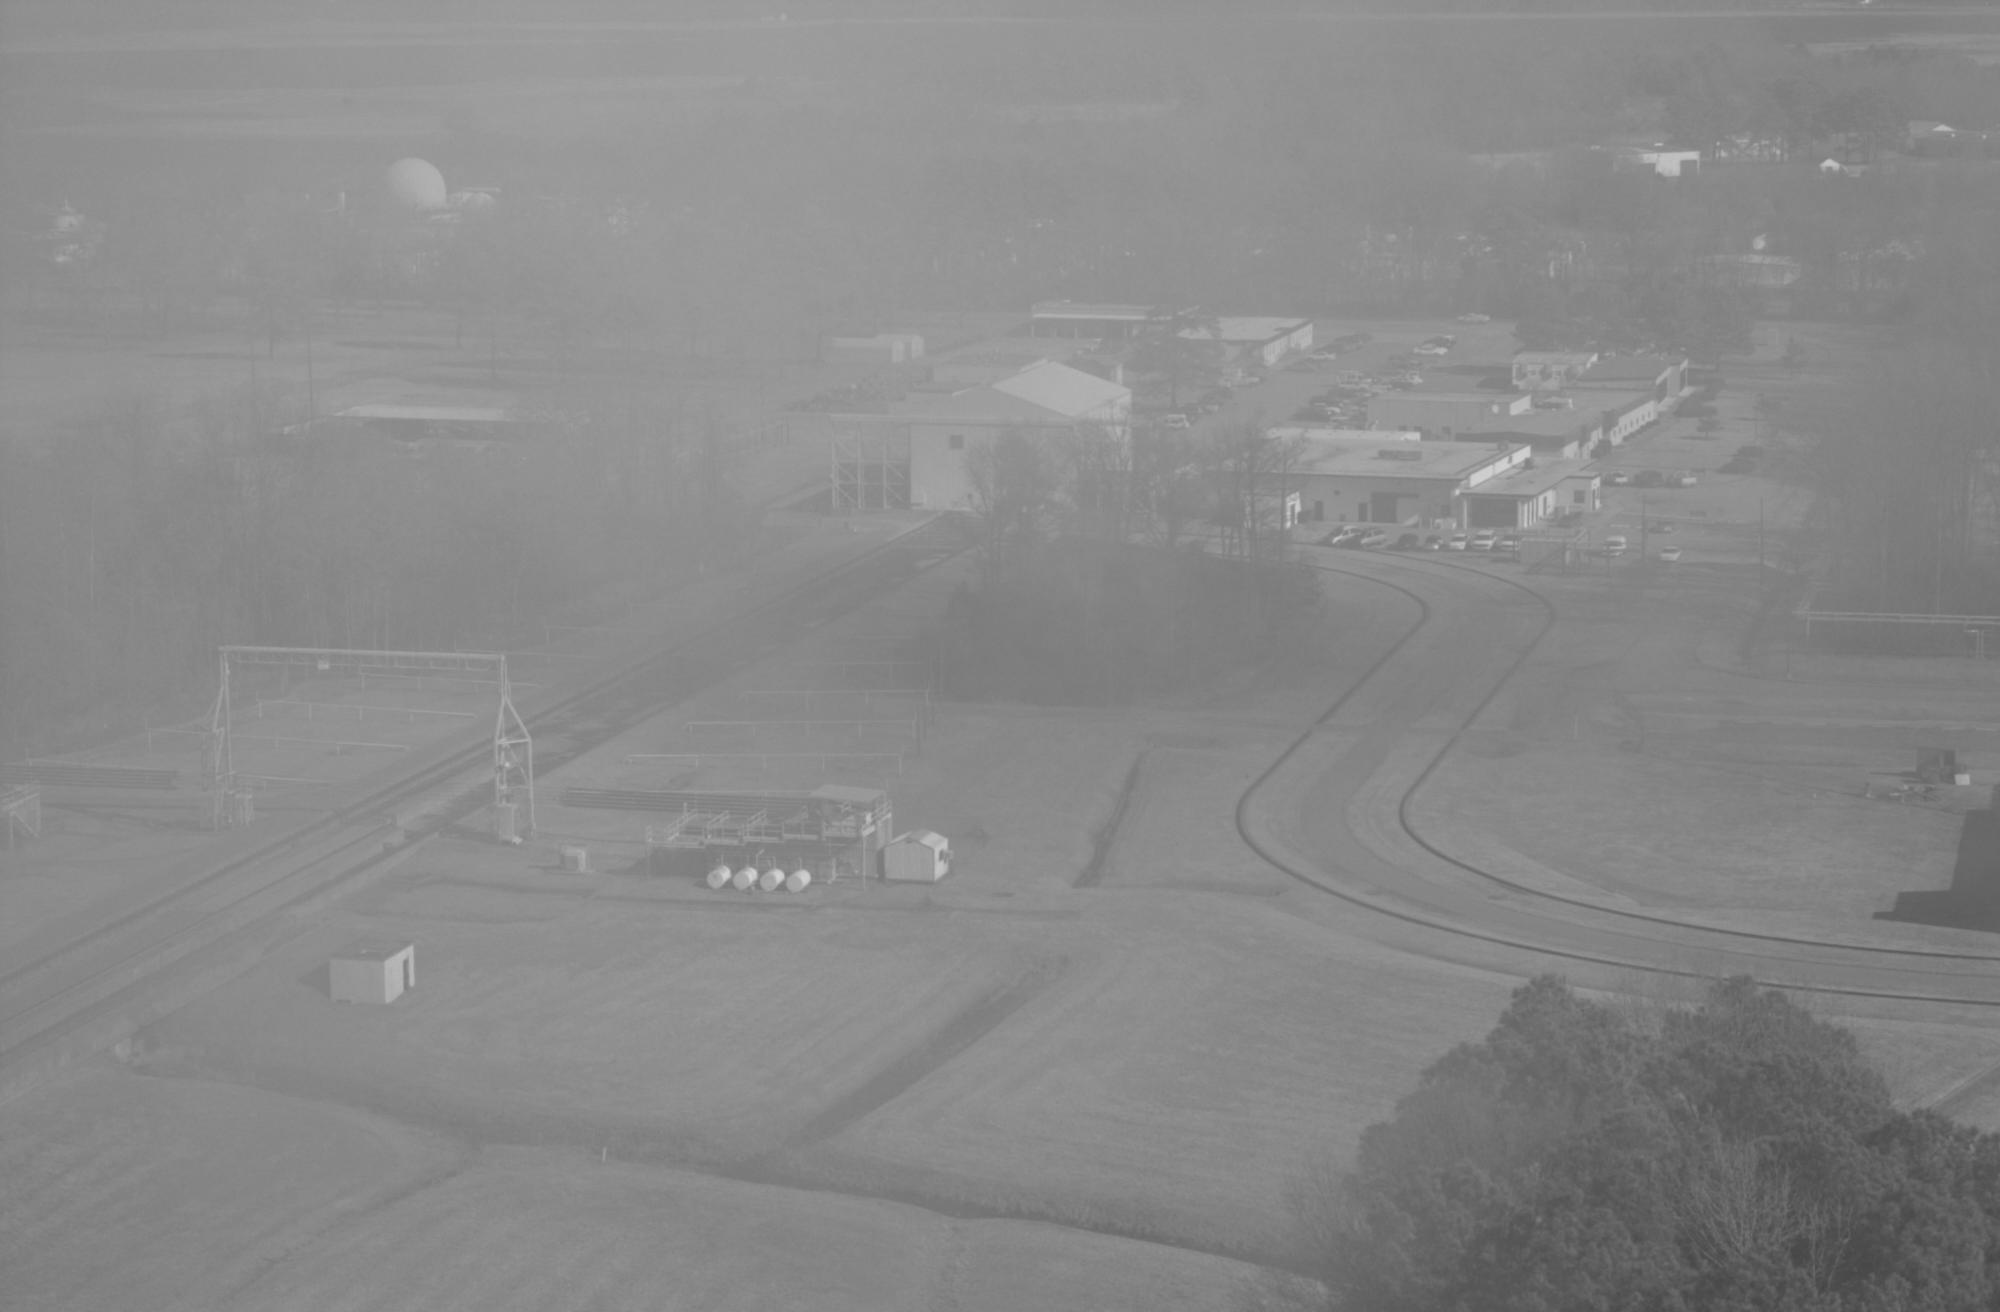
\includegraphics[width=\textwidth]{figs/lc2_gray}
		\caption{original}
		\label{fig:lc2_orig}
	\end{subfigure}
	
	\begin{subfigure}[h]{0.75\textwidth}
		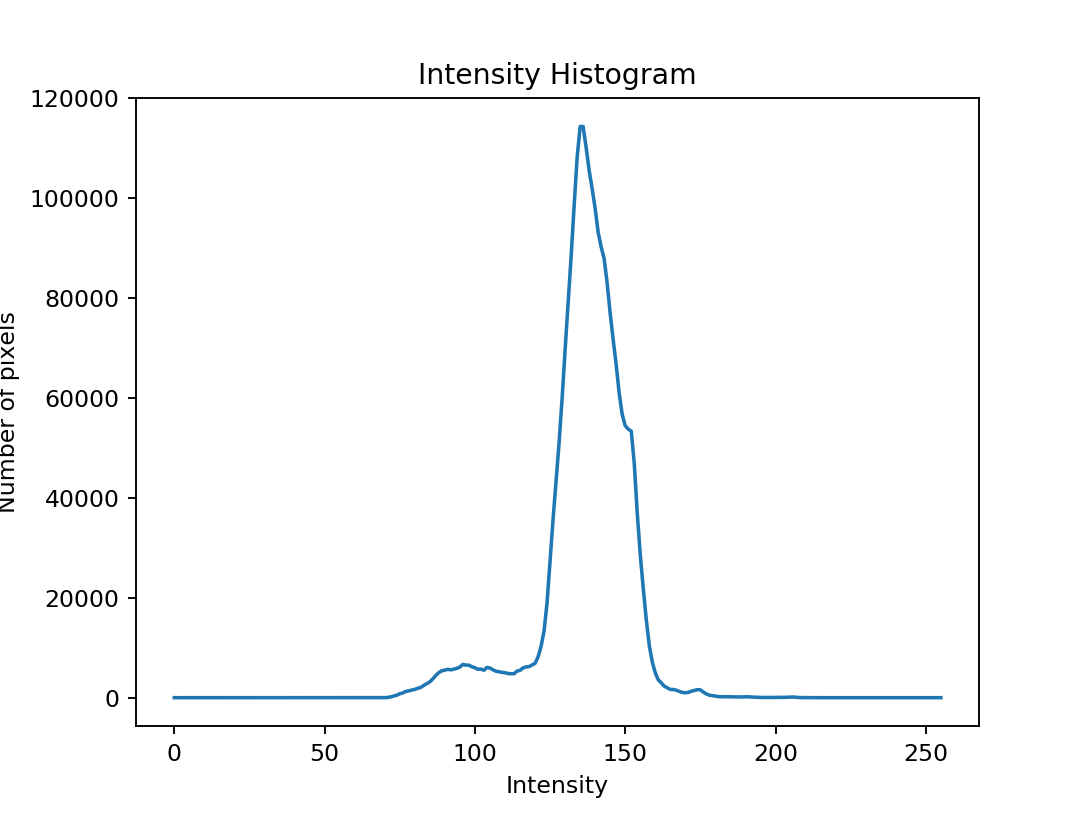
\includegraphics[width=\textwidth]{figs/lc2_hist_bef}
		\caption{before}
		\label{fig:hist_bef_2}
	\end{subfigure}
	
	\caption{Contrast enhancement.}
	\label{fig:eq2}
\end{figure}

\clearpage

\begin{figure}[h]
	\ContinuedFloat
	\centering
	\begin{subfigure}[h]{0.7\textwidth}
		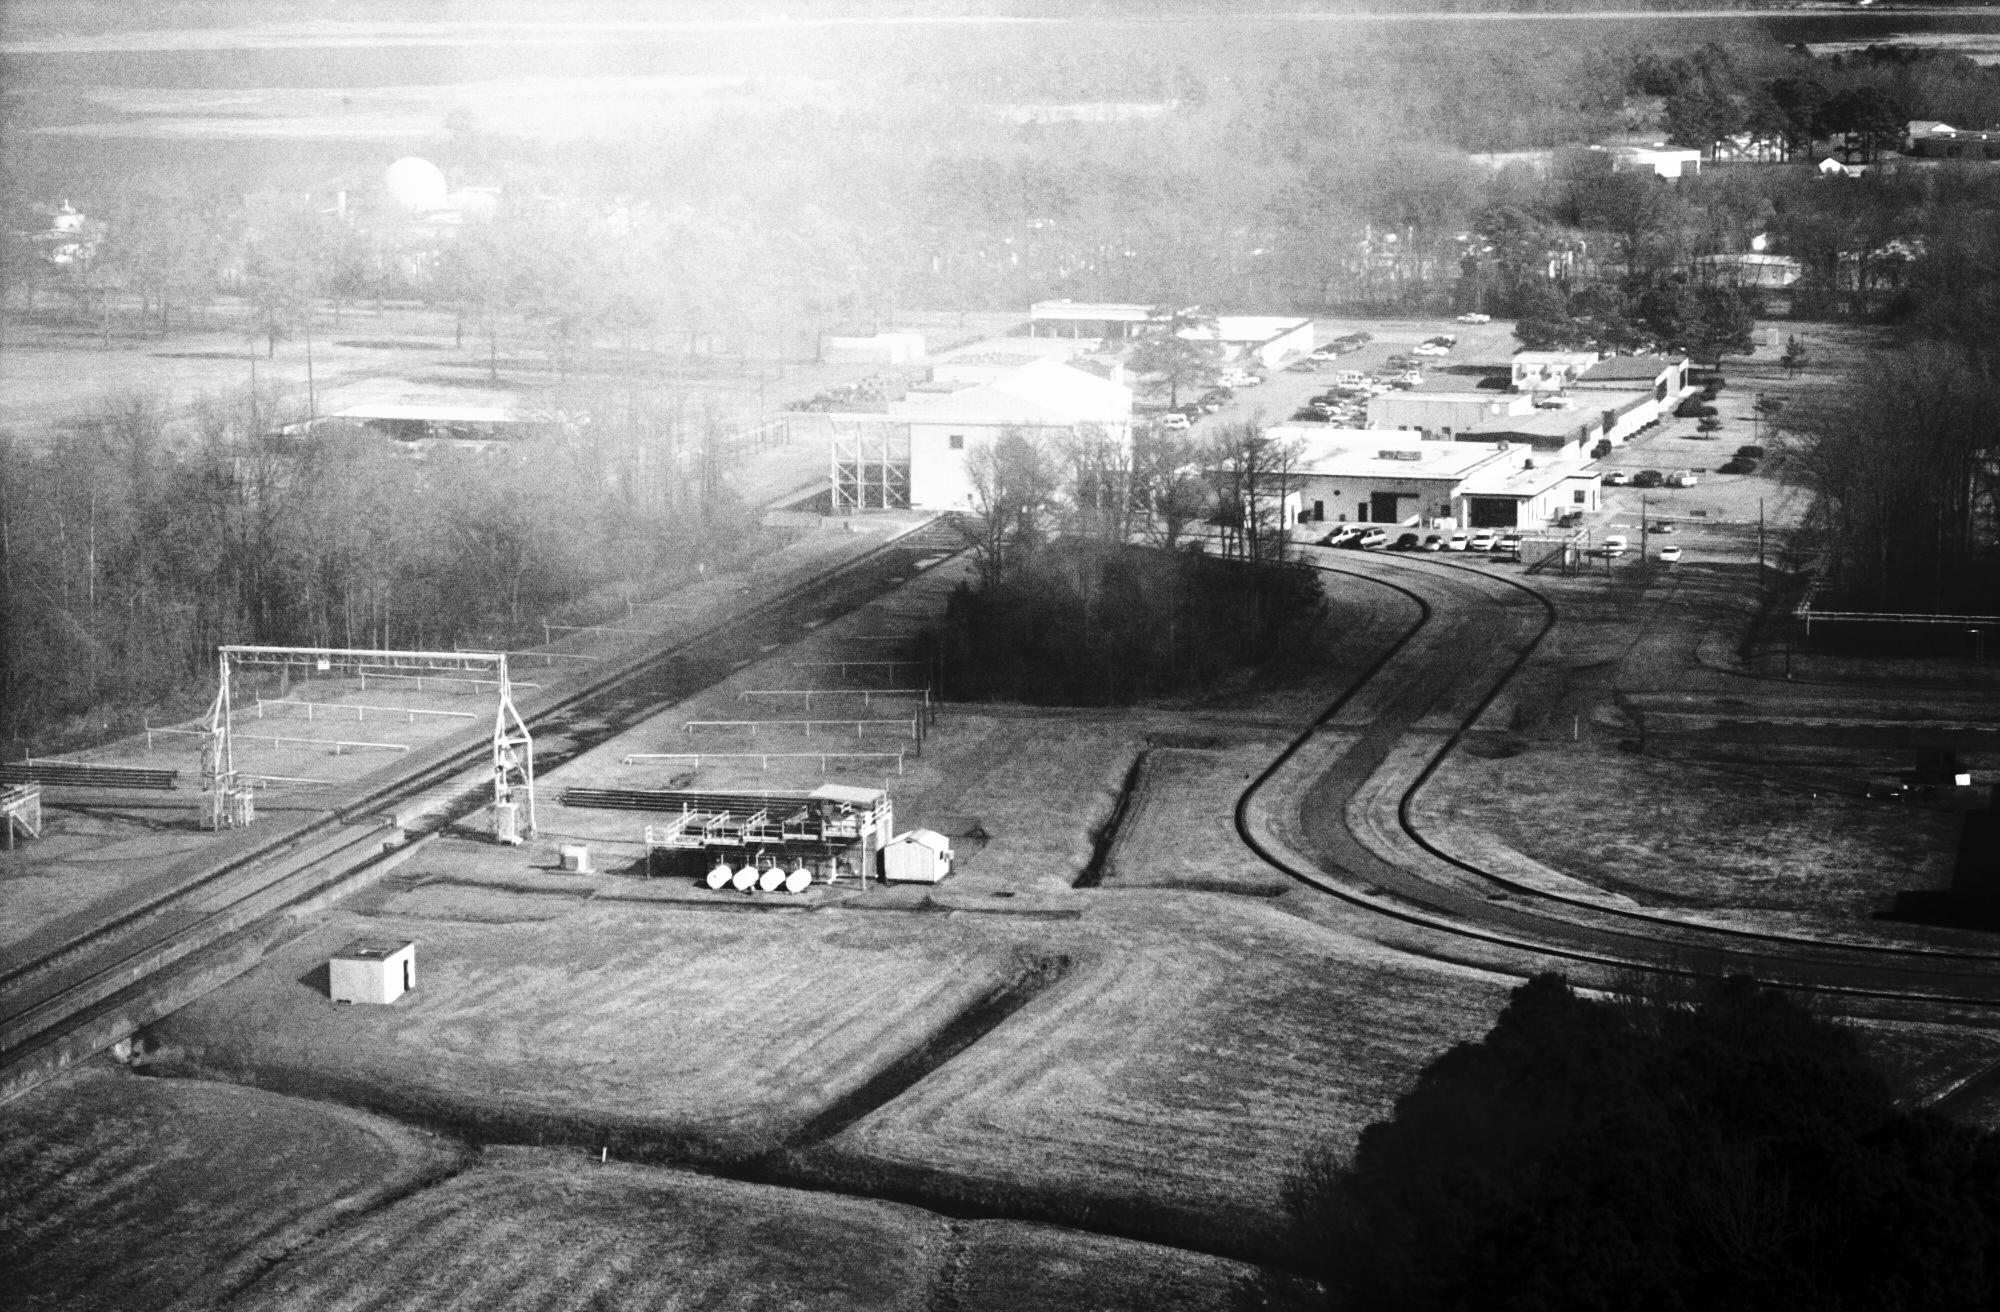
\includegraphics[width=\textwidth]{figs/lc2_ce}
		\caption{contrast enhanced}
		\label{fig:lc2_after}
	\end{subfigure}
	
	\begin{subfigure}[h]{0.75\textwidth}
		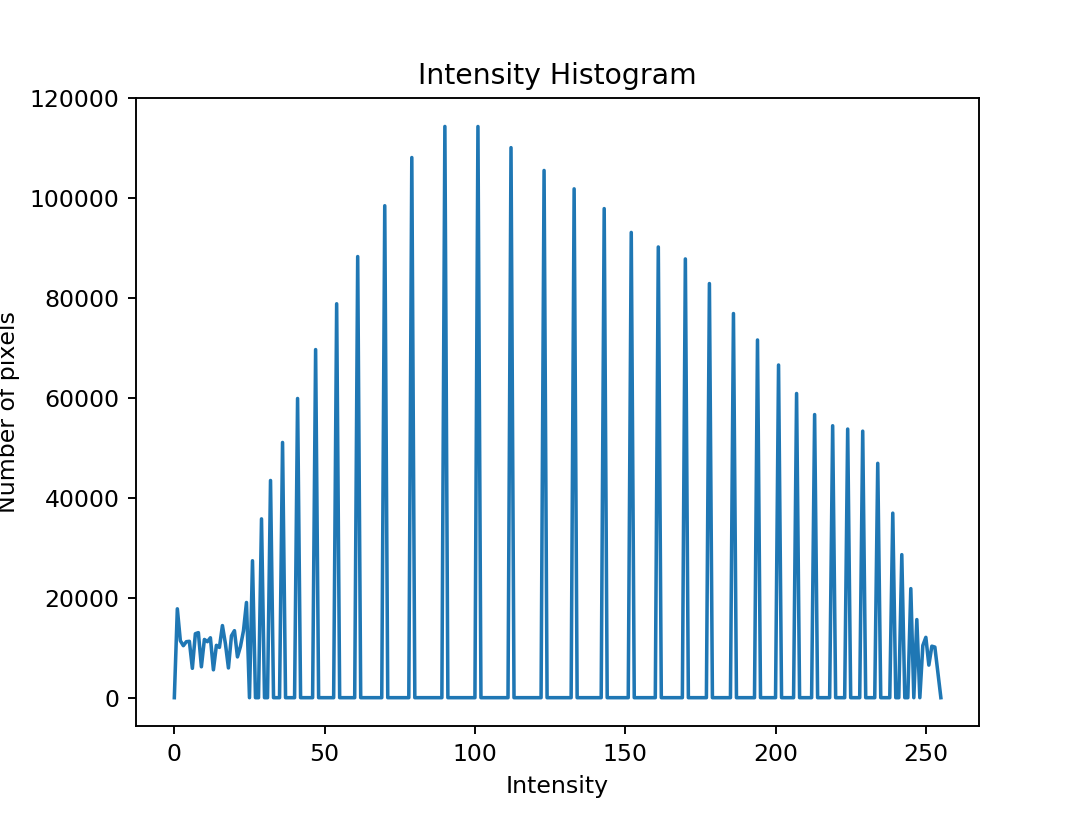
\includegraphics[width=\textwidth]{figs/lc2_hist_aft}
		\caption{after}
		\label{fig:hist_aft_2}
	\end{subfigure}
\end{figure}

\clearpage







\pagebreak

\section{Appendix}

\subsection{Appendix A: Main} \label{app:main}
	\begin{lstlisting}[language=Python,label={lst:main}]
	
	\end{lstlisting}
	
\subsection{Appendix B: Grayscale Conversion} \label{app:gray}
	\begin{lstlisting}[language=Python,label={lst:gray}]
def grayscale(image):
    imageIn = np.asarray(image,np.uint8)
    rows = imageIn.shape[0]
    cols = imageIn.shape[1]

    # convert image to grayscale
    Y = [0.299,0.587,0.114]
    imGray = np.dot(imageIn,Y)
    imGray = imGray.astype(np.uint8)

    # convert ndarray into linear array
    linIm = np.reshape(imGray,rows * cols)

    # clip out of bounds values
    linIm = np.where(linIm < 0,0,linIm)
    linIm = np.where(linIm > 255,255,linIm)

    # reshape back into 2D array
    imGray = np.reshape(linIm,[rows,cols])

    return imGray
	\end{lstlisting}
	
\subsection{Appendix C: Histogram Equalization}
	\begin{lstlisting}[language=Python,label={lst:hist}]
def histEQ(image):
    image = image.convert('L')
    image = np.asarray(image, np.float)
    hist_before = np.zeros(256, dtype=int)
    freq = Counter(np.reshape(image, image.shape[0] * image.shape[1]))
    for p in range(256):
        hist_before[p] = freq[p]
    remap = np.zeros(256, dtype=int)
    remap[-1] = 255
    histSum = sum(hist_before[1:-2])
    P = histSum / 254
    T = P
    outval = 1
    curr_sum = 0
    # build remap table
    for inval in range(1, 255, 1):
        curr_sum += hist_before[inval]
        remap[inval] = outval
        if (curr_sum > T):
            outval = round(curr_sum/P)
            T = outval*P
    # declare output image
    image_equalized = np.zeros_like(image)
    # remap intensities into equalized array
    for intensity in range(256):
        # remap values to equalize
        image_equalized = np.where(image == intensity, remap[intensity], image_equalized)
    # compute histogram after equalization
    hist_after = np.zeros(256,dtype=int)
    freq = Counter(np.reshape(image_equalized,image_equalized.shape[0] * image_equalized.shape[1]))
    for p in range(256):
        hist_after[p] = freq[p]
    return image_equalized, hist_before, hist_after, remap, image
    \end{lstlisting}

\end{document}